\chapter{FEM.js}
\label{cha:FEM.js}

FEM.js es una aplicación web desarrollada con Three.js; una \emph{API} programada en JavaScript para crear escenas tridimensionales en el navegador web, para modelar estructuras aporticadas sometidas a cargas estáticas. Una copia del programa se encuentra alojada en la página web de GitHub \url{https://github.com/rvcristiand/FEM.js}.\\

Los archivos principales de la aplicación web son:\\

\dirtree{%
  .1 FEM.js/.
  .2 LICENSE.
  .2 README.md.
  .2 css/.
  .3 style.css.
  .2 example\_1.json.
  .2 example\_2.json.
  .2 example\_3.json.
  .2 index.html.
  .2 libs/.
  .3 CSS2DRenderer.js.
  .3 OrbitControls.js.
  .3 Projector.js.
  .3 dat.gui.min.js.
  .3 stats.js.
  .3 three.js.
  .2 main.js.
  .2 modules/.
  .3 FEM.js.
  .3 terminal.js.
}
\bigskip

El usuario puede acceder al programa visitando la página web \url{https://rvcristiand.github.io/FEM.js}, o a través de un \emph{servidor local}, para modelar estructuras aporticadas tridimensionales sometidas a cargas estáticas. En la figura \ref{fig:FEM.js} se presenta FEM.js ejecutándose por primera vez en el navegador web Firefox.\\

\begin{figure}[ht]
    \centering
    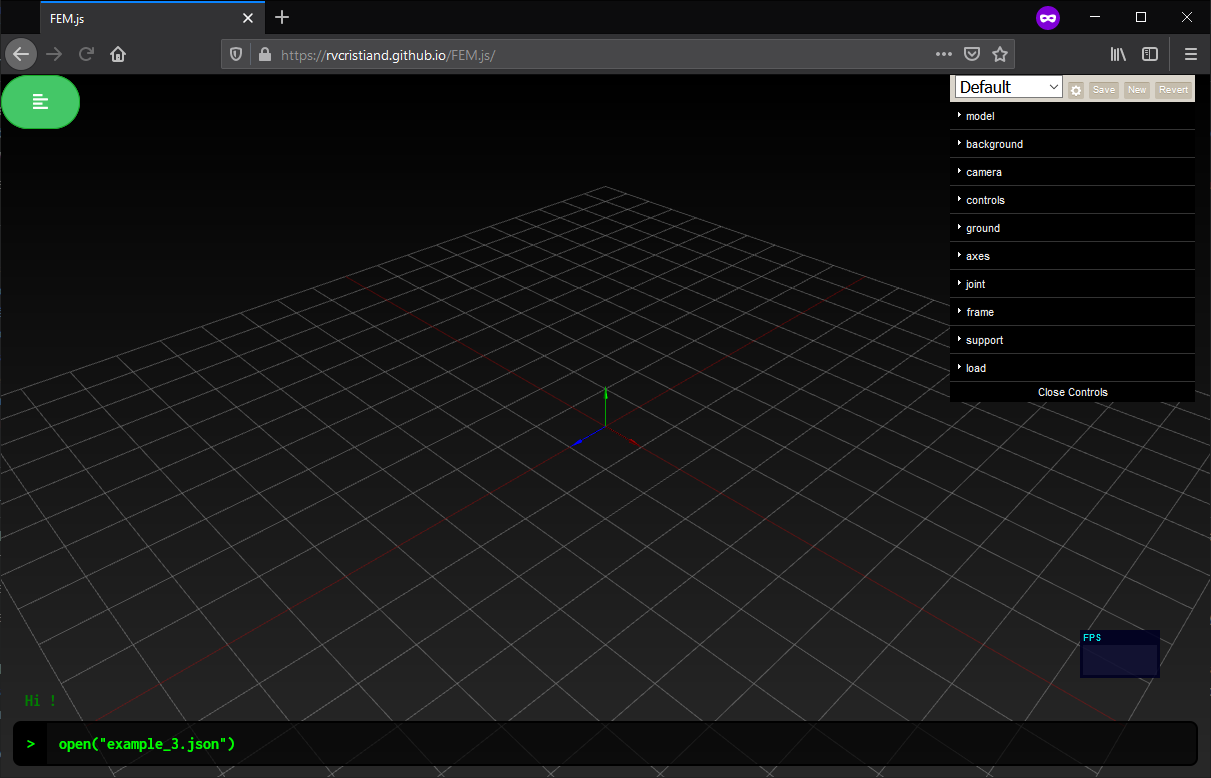
\includegraphics[width=0.8\textwidth]{FEM.js/FEM.js.png}
    \caption{FEM.js ejecutándose en el navegador web Firefox.}
    \label{fig:FEM.js}
\end{figure}

Una vez toda la aplicación web ha sido descargada se ejecuta la función \verb|init()|, definida en el archivo \verb|FEM.js|, para desplegar la página web según ciertos valores por defecto, o los que el usuario previamente haya guardado (a través del panel superior de la barra de herramientas), almacenados en la variable \verb|config|.\\

En el algoritmo \ref{alg:FEM.js-init} se presenta el pseudocódigo de la función \verb|init()|. Inicialmente la función actualiza los valores por defecto con los que el usuario haya guardado, y con ellos configura la escena tridimensional y algunos elementos asociados a esta, como las luces de la escena o los materiales con los cuales se van a representar los elementos del modelo.\\

Después crea un nuevo modelo con la función \verb|createModel()|, lo rota con la función \verb|setModel| \verb|Rotation()|, de tal manera que uno de los ejes principales del modelo queda apuntando hacia la parte superior de la pantalla, y lo agrega a la escena con el método \verb|add()|. Algo similar hace para agregar un plano horizontal a la escena.\\

Finalmente, crea una nueva estructura con la función \verb|createStructure()| para almacenar la información del modelo, un monitor para medir el desempeño de la aplicación, la barra de herramientas y ejecuta la función \verb|render()|.\\

\begin{lstlisting}[language={},caption=Pseudocódigo de la función \texttt{init()} del archivo \texttt{FEM.js}.,label=alg:FEM.js-init,frame=single]
function init() {
  // refresh the config
  
  // set the background
  
  // create the scene
  
  // create the camera

  ...
  
  // create the controls
  
  // set the materials
  
  // create the model
  model = createModel();
  setModelRotation( config[ 'model.axisUpwards' ] );
  scene.add( model );
  
  // create the ground
  var ground = createGround( config[ 'ground.size' ], config[ 'ground.grid.divisions' ], config[ 'ground.plane.color' ], config[ 'ground.plane.transparent' ], config[ 'ground.plane.opacity' ], config[ 'ground.grid.major' ], config[ 'ground.grid.minor' ] );
  scene.add( ground );
  
  // create the structure
  structure = createStructure();

  // create the stats

  // create the dat gui

  render();
}
\end{lstlisting}
\bigskip

Los valores por defecto que usa FEM.js para configurar la escena se encuentran almancenados en la variable \verb|config| del archivo \verb|FEM.js|. En el algoritmo \ref{alg:FEM.js-config} se presentan algunas entradas de dicha variable.\\

\begin{lstlisting}[language={},caption=Valores por defecto para configurar FEM.js.,label=alg:FEM.js-config,frame=single]
var config = {
  // background
  'background.topColor': '#000000',
  'background.bottomColor': '#282828',
  
  // model
  'model.axisUpwards': 'y',
  
  'model.axes.visible': true,
  'model.axes.size': 1,
  
  'model.axes.head.radius': 0.04,
  'model.axes.head.height': 0.3,
  
  'model.axes.shaft.length': 0.7, 
  'model.axes.shaft.radius': 0.01,
  
  // camera
  'camera.type': 'perspective',
  
  'camera.perspective.fov': 45,
  'camera.perspective.near': 0.1,
  'camera.perspective.far': 1000,
  
  'camera.position.x': 10,
  'camera.position.y': 10,
  'camera.position.z': 10,
  
  'camera.target.x': 0, 
  'camera.target.y': 0,
  'camera.target.z': 0,
  
  // controls
  ...
  
  // axes
  ...

  // ground
  ...
  
  // joint
  ...

  // frame
  ...
  
  // support
  ...
  
  // load
  ...
};  
\end{lstlisting}
\bigskip

A través de la barra de herramientas el usuario es capaz de modificar la mayoria de estos valores para cambiar los diferentes elementos que componen la escena tridimensional. Por ejemplo, en la figura \ref{fig:FEM.js-background} se presenta FEM.js con unos colores del fondo de la escena alternativos a los valores estándar, modificados con los controles \verb|top| y \verb|bottom| de la sección \verb|background| de la barra de herramientas.\\

\begin{figure}[ht]
  \centering
  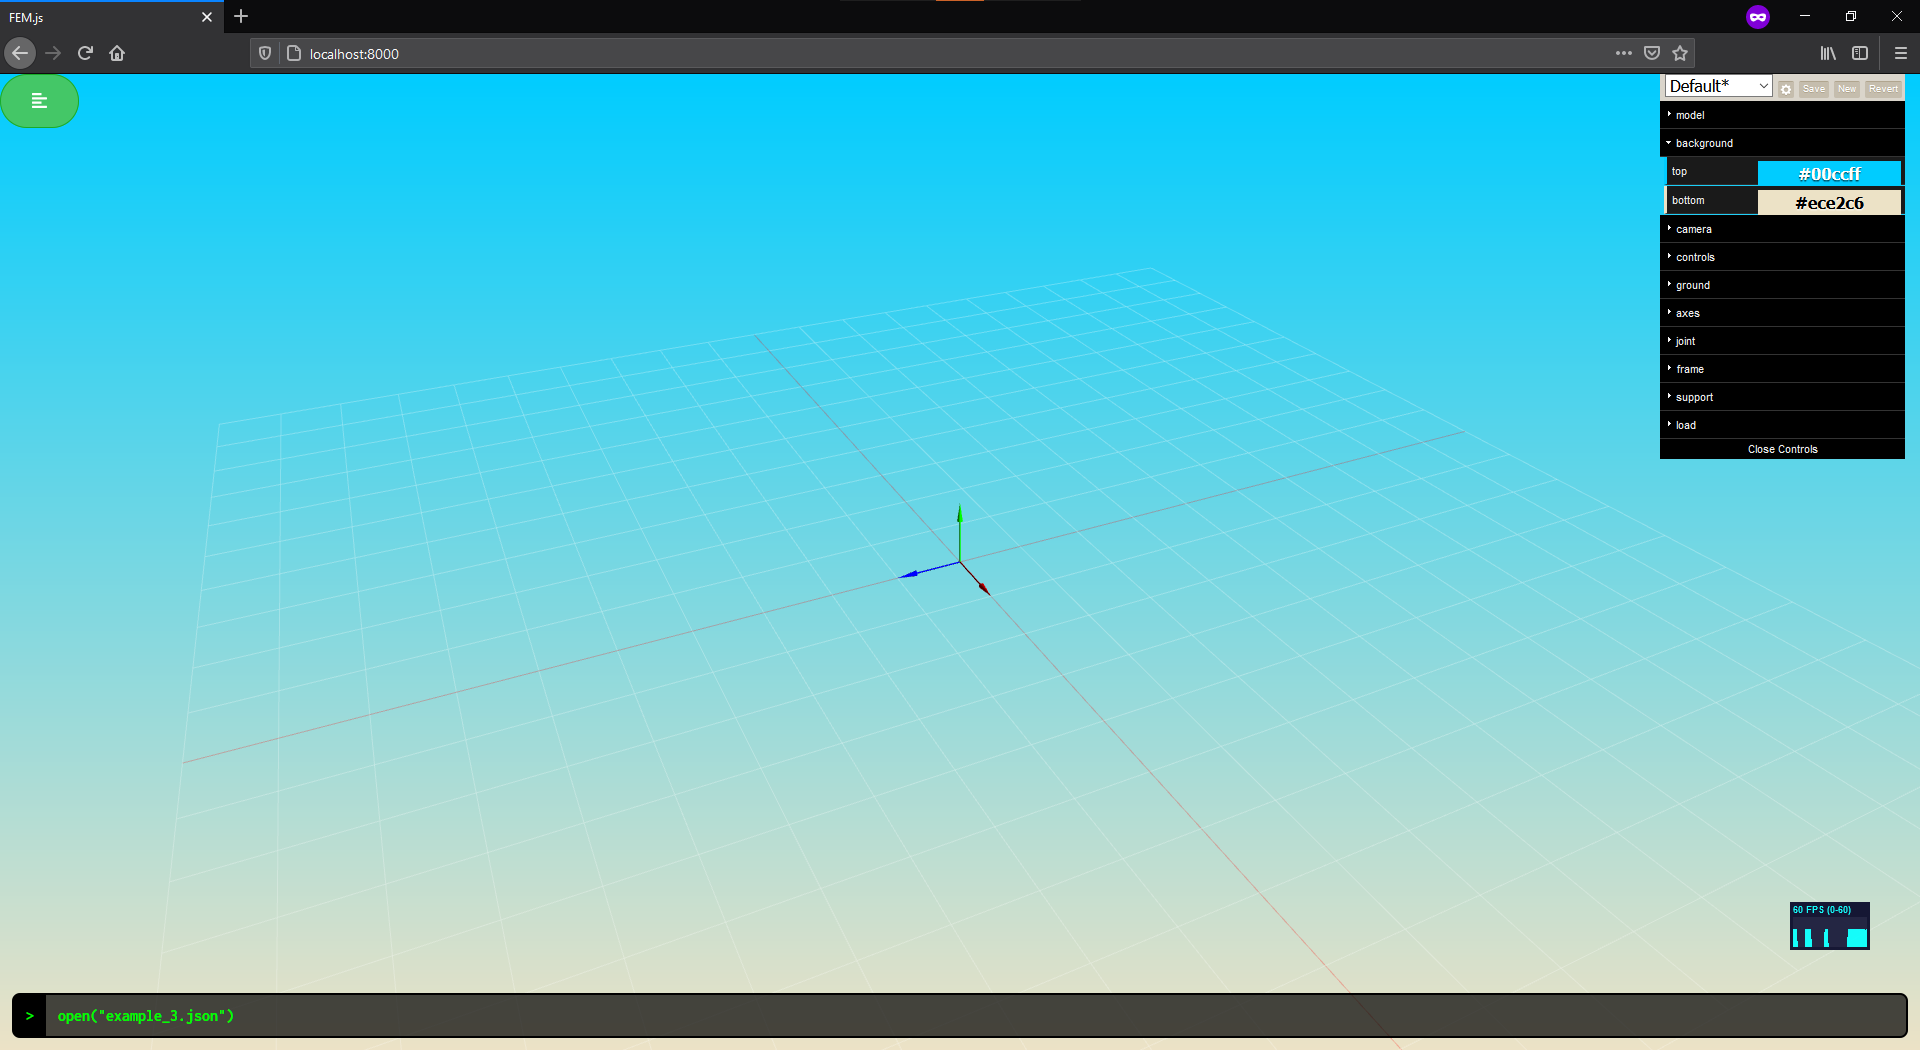
\includegraphics[width=0.8\textwidth]{FEM.js/dat-gui.png}
  \caption{FEM.js con colores del fondo de la escena arbitrarios.}
  \label{fig:FEM.js-background}
\end{figure}

El usuario puede generar múltiples configuraciones de estas opciones a través del panel superior de la barra de herramientas. Haciendo clic sobre el botón con un piñón puede copiar el objeto que describe sus configuraciones, para posteriormente configurar la aplicación web en otro dispositivo, o guardar la configuración en la variable \verb|localStorage| para ser usadas en próximas sesiones.\\

En la figura \ref{fig:FEM.js-user-preferences} se presenta FEM.js después de haber hecho clic sobre el botón con un piñon e indicando que se guarden las configuraciones en la variable \verb|localStorage|.\\

\begin{figure}[h!]
  \centering
  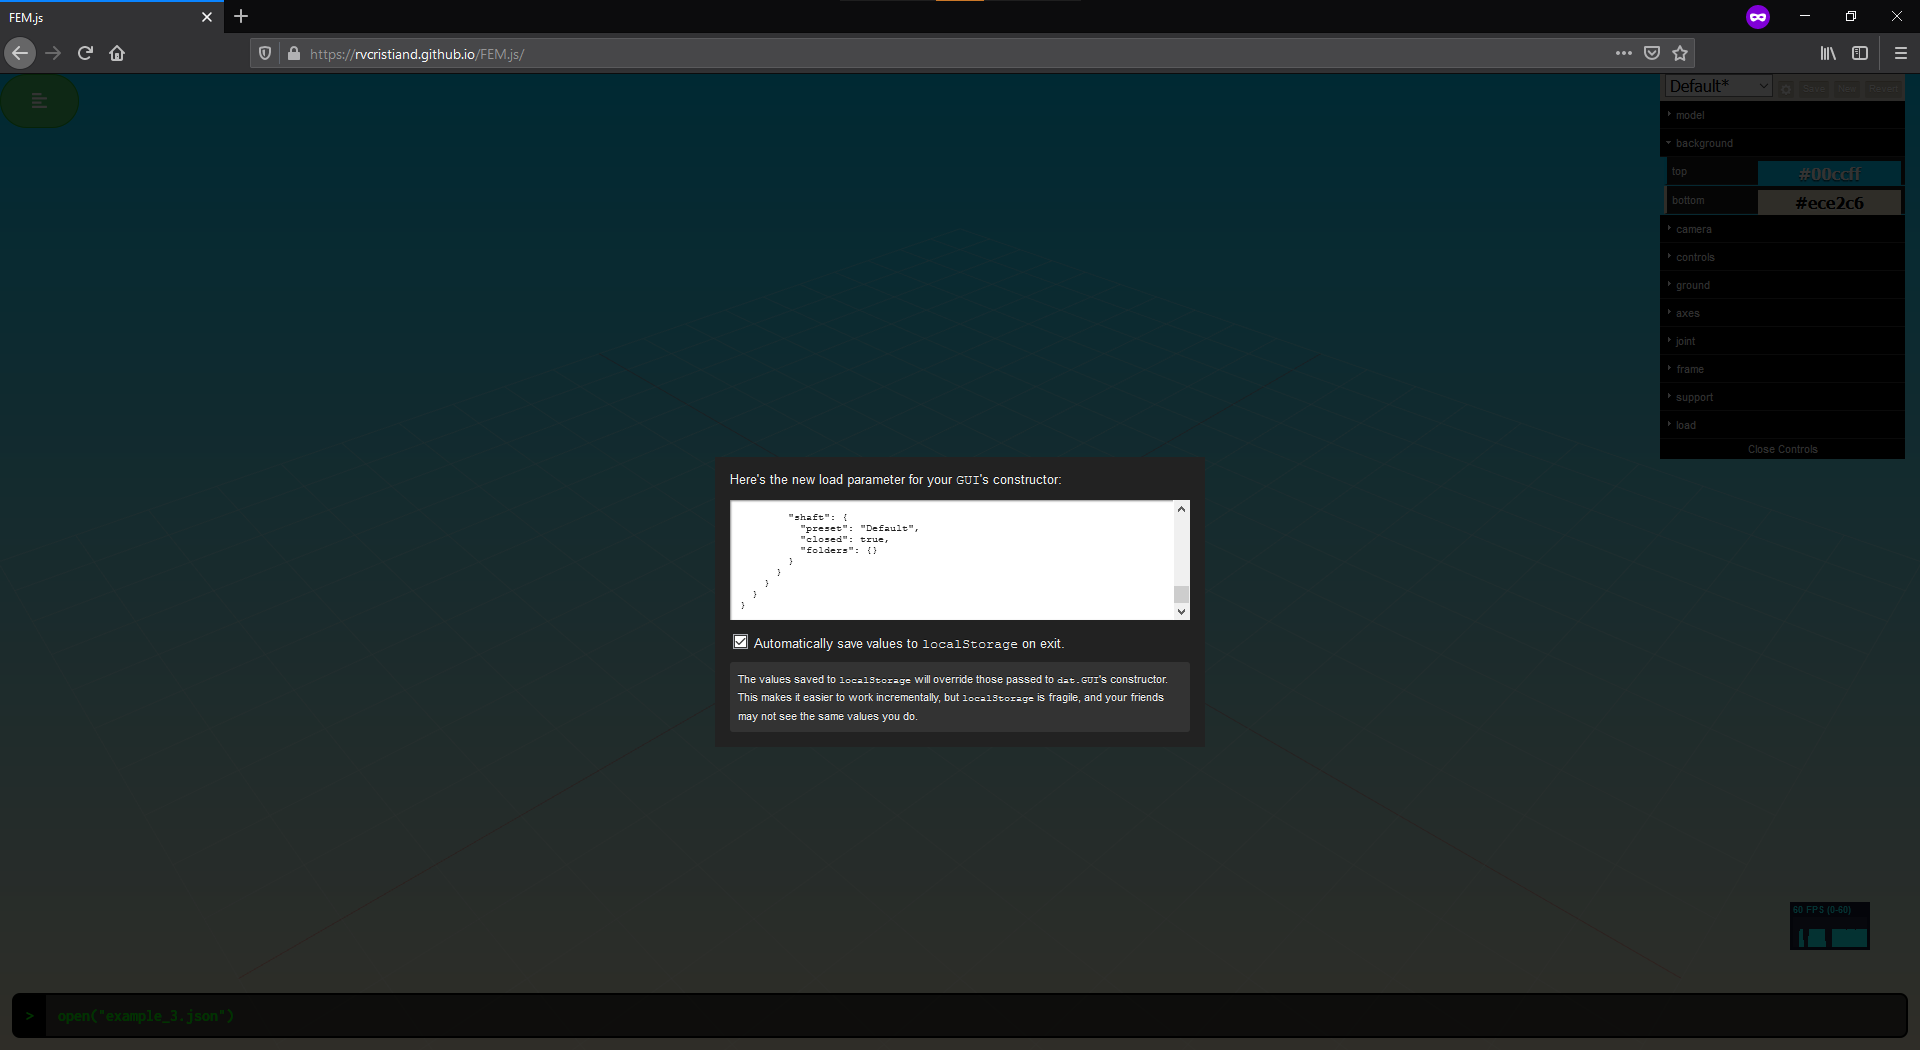
\includegraphics[width=0.8\textwidth]{FEM.js/dat-gui-user-preferences.png}
  \caption{FEM.js almacenando la configuración del usuario en la variable \texttt{localStorage}.}
  \label{fig:FEM.js-user-preferences}
\end{figure}

En el algoritmo \ref{alg:FEM.js-createModel} se presenta la implementación de la función \verb|createModel()|. La función genera un objeto tipo \verb|THREE.Group| al cual se le ha agregado los objetos \verb|axes|, \verb|joints|, \verb|frames| y \verb|loads|, también objetos tipo \verb|THREE.Group|, mediante el método \verb|add()|.\\

Según \cite{threejs-Object3D}, \verb|THREE.Object3D| es la clase base de la mayoría de los objetos en Three.js, al proveer un conjunto de métodos y propiedades para manipular objetos en la escena tridimensional. La clase \verb|THREE.Group| es casi identica que la clase \verb|THREE.Object3D|. Su proposito es permitir trabajar con grupos de objetos de manera sintáctica más clara.\\
\pagebreak

\begin{lstlisting}[language={},caption=Implementación de la función \texttt{createModel()} del archivo \texttt{FEM.js}.,label=alg:FEM.js-createModel,frame=single]
function createModel() {
  // create the model

  var model = new THREE.Group();
  model.name = "model";

  // add axes
  var axes = createAxes( config[ 'model.axes.shaft.length' ], config[ 'model.axes.shaft.radius'], config[ 'model.axes.head.height'], config[ 'model.axes.head.radius'] );
  axes.name = 'axes';
  axes.visible = config[ 'model.axes.visible' ];
  axes.scale.setScalar( config[ 'model.axes.size' ] );
  model.add( axes );
  
  // add joints
  var joints = new THREE.Group();
  joints.name = 'joints';
  model.add( joints );
  
  // add frames
  var frames = new THREE.Group();
  frames.name = 'frames';
  frames.visible = config[ 'frame.visible' ];
  model.add( frames );

  // add loads
  var loads = new THREE.Group();
  loads.name = 'loads';
  loads.visible = config[ 'load.visible' ];
  model.add( loads );

  return model;
}
\end{lstlisting}
\bigskip

En el algoritmo \ref{alg:FEM.js-createStructure} se presenta la implementación de la función \verb|createStructure()|. La función crea un nuevo objeto con las entradas \verb|joints|, \verb|materials|, \verb|sections|, \verb|frames|, \verb|supports| y \verb|load_patterns|.\\

\begin{lstlisting}[language={},caption=Implementación de la función \texttt{createStructure()} del archivo \texttt{FEM.js}.,label=alg:FEM.js-createStructure,frame=single]
function createStructure() { return { joints: {}, materials: {}, sections: {}, frames: {}, supports: {}, load_patterns: {} } };
\end{lstlisting}
\bigskip

En el algoritmo \ref{alg:FEM.js-render} se presenta la implementación de la función \verb|render()|. Esta función se llama así mismo cada cierto tiempo, mediante la función \verb|requestAnimationFrame()|, para repintar la escena tridimensional, actualizar el monitor de desempeño y los controles de la cámara, de ser necesario.\\

Según \cite{MDNWebDocs-requestAnimationFrame}, la función \verb|requestAnimationFrame()| le indica al navegador web que se desea hacer una animación y se requiere llamar una función en específico (en este caso la función \verb|render()|) que actualice la animación antes de la siguiente repintada. En general, la función es ejecutada 60 veces por segundo.\\

\begin{lstlisting}[language={},caption=Implementación de la función \texttt{render()} del archivo \texttt{FEM.js}.,label=alg:FEM.js-render,frame=single]
function render() {
  // render the scene

  requestAnimationFrame( render );

  stats.update();

  webGLRenderer.render( scene, camera );
  CSS2DRenderer.render( scene, camera );

  if ( controls.enableDamping ) controls.update();
}
\end{lstlisting}
\bigskip

Una vez la aplicación web está desplegada, el usuario puede comenzar a modelar la estructura ejecutando un conjunto de funciones a través de la línea de comandos de FEM.js. Dicho conjunto de funciones están listadas en el archivo \verb|main.js|, aunque la implementación de las mismas se encuetran en el archivo \verb|FEM.js|.\\

Estas funciones tienen por objeto modificar las variables \verb|model| y \verb|structure|, las cuales almacena los objetos tridimensionales del modelo y su información, respectivamente. A continuación se presenta la implementación de cada una de estas funciones.\\

\section{open()}

La función \verb|open()| permite abrir archivos con modelos de estructuras almacenados en formato JSON. La función recibe el nombre del archivo, y mediante un conjunto de funciones creadas para tal fin, lee cada uno de los objetos allí almacenados y los agrega al programa.\\

En el algoritmo \ref{alg:FEM.js-open} se presenta el pseudocódigo de la función \verb|open()|. Esta función elimina cualquier objeto que se le haya agregado a la variable \verb|model| y le asigna un nuevo objeto a la variable \verb|structure|, con la función \verb|createStructure()| (véase el algoritmo \ref{alg:FEM.js-createStructure}), antes de agregar cada uno de los objetos definidos en el archivo indicado por el usuario.\\

\begin{lstlisting}[language={},caption=Implementación de la función \texttt{open()} del archivo \texttt{FEM.js}.,label=alg:FEM.js-open,frame=single]
export function open( filename ) {
  // open a file

  var promise = loadJSON( filename )
    .then( json => {
      // delete labels
      ...
      
      // delete objects
      ...

      // create structure
      structure = createStructure();
      
      // add materials
      ...

      // add sections
      ...

      // add joints
      ...

      // add frames
      ...

      // add suports
      ...

      // add load patterns
      ...

      return "the '" + filename + "' model has been loaded";
    });

  return promise;
}
\end{lstlisting}
\bigskip

En la figura \ref{fig:FEM.js-example_2} se presenta FEM.js después de ejecutar la función \verb|open()| para abrir el archivo \verb|example_2.json|. Este archivo ha sido generado con pyFEM, un programa de computador desarrollado en Python para analizar estructuras aporticadas sometidas a cargas estáticas, para analizar el ejercicio 7.2 de \cite{escamilla1995microcomputadores}.\\

A través de la barra de herramientas el usuario puede modificar la aparencia de los objetos que se muestran en la escena. Para este caso en particular, se le indicó a FEM.js que mostrara los nombres de los nodos, los cuales se presentan en blanco sobre un rectángulo negro, y que ocultara los ejes locales de los elementos aporticados.\\

\begin{figure}[ht]
  \centering
  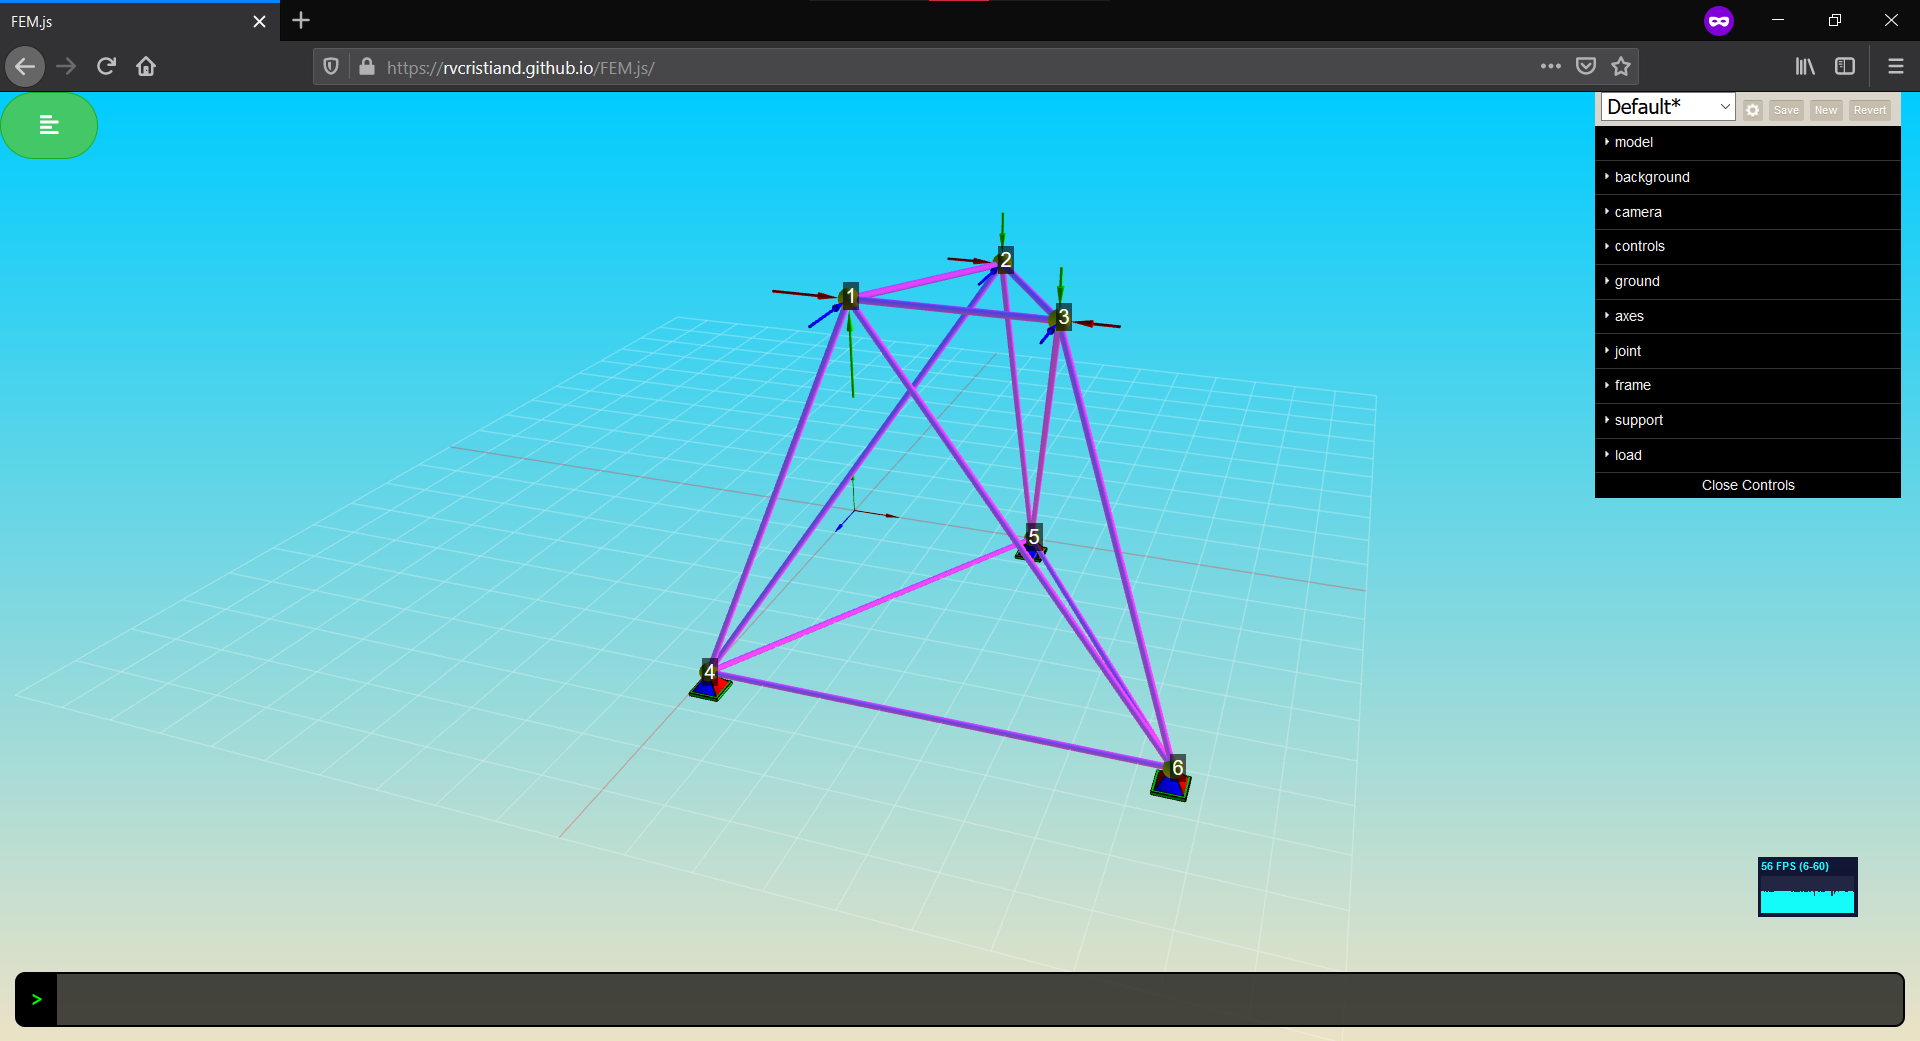
\includegraphics[width=0.8\textwidth]{FEM.js/FEM.js-example_2.png}
  \caption{Archivo \texttt{example\_2.json} abierto con FEM.js.}
  \label{fig:FEM.js-example_2}
\end{figure}

A continuación se presenta el contenido del archivo \verb|example_2.json|. FEM.js lee los materiales, secciones transversales, nodos, elementos aporticados y los patrones de carga, los agrega a la variable \verb|structure| y crea su correspondiente representación en la escena, mediante una serie de funciones desarrolladas para tal fin.\\

\begin{lstlisting}[language={},multicols=2]
{
  "materials": {
      "2100 t/cm2": {
          "E": 21000000.0,
          "G": 0
      }
  },
  "sections": {
      "10 cm2": {
          "area": 0.001,
          "Ix": 0,
          "Iy": 0,
          "Iz": 0,
          "type": "Section"
      },
      "20 cm2": {
          "area": 0.002,
          "Ix": 0,
          "Iy": 0,
          "Iz": 0,
          "type": "Section"
      },
      "40 cm2": {
          "area": 0.004,
          "Ix": 0,
          "Iy": 0,
          "Iz": 0,
          "type": "Section"
      },
      "50 cm2": {
          "area": 0.005,
          "Ix": 0,
          "Iy": 0,
          "Iz": 0,
          "type": "Section"
      }
  },
  "joints": {
      "1": {
          "x": 2.25,
          "y": 6,
          "z": 4.8
      },
      "2": {
          "x": 3.75,
          "y": 6,
          "z": 2.4
      },
      "3": {
          "x": 5.25,
          "y": 6,
          "z": 4.8
      },
      "4": {
          "x": 0.0,
          "y": 0,
          "z": 6.0
      },
      "5": {
          "x": 3.75,
          "y": 0,
          "z": 0.0
      },
      "6": {
          "x": 7.5,
          "y": 0,
          "z": 6.0
      }
  },
  "frames": {
      "1-2": {
          "j": "1",
          "k": "2",
          "material": "2100 t/cm2",
          "section": "20 cm2"
      },
      "1-3": {
          "j": "1",
          "k": "3",
          "material": "2100 t/cm2",
          "section": "20 cm2"
      },
      "1-4": {
          "j": "1",
          "k": "4",
          "material": "2100 t/cm2",
          "section": "40 cm2"
      },
      "1-6": {
          "j": "1",
          "k": "6",
          "material": "2100 t/cm2",
          "section": "50 cm2"
      },
      "2-3": {
          "j": "2",
          "k": "3",
          "material": "2100 t/cm2",
          "section": "20 cm2"
      },
      "2-4": {
          "j": "2",
          "k": "4",
          "material": "2100 t/cm2",
          "section": "50 cm2"
      },
      "2-5": {
          "j": "2",
          "k": "5",
          "material": "2100 t/cm2",
          "section": "40 cm2"
      },
      "3-5": {
          "j": "3",
          "k": "5",
          "material": "2100 t/cm2",
          "section": "50 cm2"
      },
      "3-6": {
          "j": "3",
          "k": "6",
          "material": "2100 t/cm2",
          "section": "40 cm2"
      },
      "4-5": {
          "j": "4",
          "k": "5",
          "material": "2100 t/cm2",
          "section": "10 cm2"
      },
      "4-6": {
          "j": "4",
          "k": "6",
          "material": "2100 t/cm2",
          "section": "10 cm2"
      },
      "5-6": {
          "j": "5",
          "k": "6",
          "material": "2100 t/cm2",
          "section": "10 cm2"
      }
  },
  "supports": {
      "4": {
          "ux": true,
          "uy": true,
          "uz": true,
          "rx": false,
          "ry": false,
          "rz": false
      },
      "5": {
          "ux": true,
          "uy": true,
          "uz": true,
          "rx": false,
          "ry": false,
          "rz": false
      },
      "6": {
          "ux": true,
          "uy": true,
          "uz": true,
          "rx": false,
          "ry": false,
          "rz": false
      }
  },
  "load_patterns": {
      "point loads": {
          "joints": {
              "1": [
                  {
                      "fx": 10,
                      "fy": 15,
                      "fz": 15,
                      "mx": 0,
                      "my": 0,
                      "mz": 0
                  }
              ],
              "2": [
                  {
                      "fx": 5,
                      "fy": -3,
                      "fz": -3,
                      "mx": 0,
                      "my": 0,
                      "mz": 0
                  }
              ],
              "3": [
                  {
                      "fx": -4,
                      "fy": -2,
                      "fz": -2,
                      "mx": 0,
                      "my": 0,
                      "mz": 0
                  }
              ]
          }
      }
  }
}
\end{lstlisting}
\bigskip

El usuario es capaz de ejecutar las mismas funciones para agregar estos elementos al programa, permitiéndole modelar sus estructuras. A continuación se presentan dichas funciones.\\

\subsection{addMaterial()}

La función \verb|addMaterial()| permite agregar materiales al programa. La función recibe los valores del módulo de Young y el módulo a cortante del material.\\

En el algoritmo \ref{alg:FEM.js-addMaterial} se presenta la implementación de la función \verb|addMaterial()|. Antes de agregar la nueva entrada a la variable \verb|structure|, la función verifica que no haya otro material con el mismo nombre.\\ 

\begin{lstlisting}[language={},caption=Función \texttt{addMaterial()} implementada en el archivo \texttt{FEM.js}.,label=alg:FEM.js-addMaterial, frame=single]
export function addMaterial( name, e, g ) {
  // add a material

  var promise = new Promise( ( resolve, reject ) => {
    // only strings accepted as name
    name = name.toString();

    // check if material's name already exits
    if ( structure.materials.hasOwnProperty( name ) ) {
      reject( new Error( "material's name '" + name + "' already exist" ) );
    } else {
      // add material to structure
      structure.materials[ name ] = { "E": e, "G": g };

      resolve( "material '" + name + "' was added" );
    }
  });

  return promise;
}
\end{lstlisting}

\subsection{addSection()}

La función \verb|addSection()| permite agregar secciones transversales generales al programa. La función recibe el nombre de la sección.\\

En el algoritmo \ref{alg:FEM.js-addSection} se presenta la implementación de la función \verb|addSection()|. Antes de agregar las nuevas entradas en las variables \verb|structure| y \verb|sections|, la función verifica que no haya otra sección transversal con el mismo nombre.\\

En ese caso, en la variable \verb|structure| se almacena la información de la sección transversal general, mientras que en la variable \verb|sections| se almacena un objeto tipo \verb|THREE.Shape| que representa un círculo de radio unitario creado con la función \verb|createSection()|.\\

Según \cite{threejs-Shape}, con los objetos tipo \verb|THREE.Shape| se pueden definir figuras planas en dos dimensiones usando \emph{paths}. Estos objetos pueden ser extrudios para crear geometrías tridimensionales.\\

\begin{lstlisting}[language={},caption=Función \texttt{addSection()} implementada en el archivo \texttt{FEM.js}.,label=alg:FEM.js-addSection, frame=single]
export function addSection( name ) {
  // add a section

  var promise = new Promise( ( resolve, reject ) => {
    // only strings accepted as name
    name = name.toString();

    // check if section's name already exits
    if ( structure.sections.hasOwnProperty( name ) ) {
      reject( new Error( "section's name '" + name + "' already exits" ) );
    } else {
      structure.sections[ name ] = { type: "Section" };
      // create section
      sections[ name ] = createSection();
  
      resolve( "section '" + name + "' was added" );
    }
  });

  return promise;
}
\end{lstlisting}
\bigskip

\subsection{addRectangularSection()}

La función \verb|addRectangularSection()| permite agregar secciones transversales rectangulares al programa. La función recibe el nombre de la sección transversal y la base y el alto de la figura.\\

En el algoritmo \ref{alg:FEM.js-addRectangularSection} se presenta la implementación de la función \verb|addRectangularSection()|. Antes de agregar las nuevas entradas en las variables \verb|structure| y \verb|section|, la función verifica que no haya otra sección transversal con el mismo nombre.\\

En tal caso, se agrega la información de la sección transversal rectángular en la variable \verb|structure|, mientras que en la variable \verb|sections| se almacena un objeto \verb|THREE.Shape| que representa un rectángulo de las dimensiones dadas, creado con la función \verb|createRectangular| \verb|Section()|.\\

\begin{lstlisting}[language={},caption=Función \texttt{addRectangularSection()} implementada en el archivo \texttt{FEM.js}.,label=alg:FEM.js-addRectangularSection, frame=single]
export function addRectangularSection( name, width, height ) {
  // add a rectangular section

  var promise = new Promise( ( resolve, reject ) => {
    // only strings accepted as name
    name = name.toString();

    // check if section's name already exits
    if ( structure.sections.hasOwnProperty( name ) ) {
      reject( new Error( "section's name '" + name + "' already exits" ) );
    } else {
      // add section to structure
      structure.sections[ name ] = { type: "RectangularSection", width: width, height: height };
      // create rectangular section
      sections[ name ] = createRectangularSection( width, height );
    
      resolve( "rectangular section '" + name + "' was added" );
    }
  });

  return promise;
}
\end{lstlisting}

\subsection{addJoint()}

La función \verb|addJoint()| permite agregar nodos al programa. La función recibe el nombre del nodo y sus coordenadas.\\

En el algoritmo \ref{alg:FEM.js-addJoint} se presenta la implementación de la función \verb|addJoint()|. Antes de agregar el nodo al programa, la función verifica que no haya otro con el mismo nombre o con las mismas coordenadas. En el caso que no haya ningún inconveniente, se agrega la información del nodo a la variable \verb|structure|, se crea un objeto tipo \verb|THREE.Group|, que se asigna a la variable \verb|parent|, y se agrega a la variable \verb|model|.\\

A este objeto se le modifica su posición, asignándole las coordenadas del nodo, y se le agrega el objeto  \verb|joint|, al cual, a su vez, se le ha agregado el objeto \verb|label|. El objeto \verb|joint|, creado con la función \verb|createJoint()|, representa el nodo con una esfera mientras que el objeto \verb|label| presenta el nombre del nodo con una etiqueta html (véase la figura \ref{fig:FEM.js-example_2}).\\

\begin{lstlisting}[language={},caption=Función \texttt{addJoint()} implementada en el archivo \texttt{FEM.js}.,label=alg:FEM.js-addJoint, frame=single]
export function addJoint( name, x, y, z ) {
  // add a joint

  var promise = new Promise( ( resolve, reject ) => {
    // only strings accepted as name
    name = name.toString();
    
    // check if joint's name or joint's coordinate already exits
    if ( structure.joints.hasOwnProperty( name ) || Object.values( structure.joints ).some( joint => joint.x == x && joint.y == y && joint.z == z ) ) {
      if ( structure.joints.hasOwnProperty( name ) ) {
        reject( new Error( "joint's name '" + name + "' already exist" ) );
      } else {
        reject( new Error( "joint's coordinate [" + x + ", " + y + ", " + z + "] already exist" )); 
      }
    } else {
      // add joint to structure
      structure.joints[ name ] = { x: x, y: y, z: z };

      // parent
      var parent = new THREE.Group();
      parent.name = name;
      parent.position.set( x, y, z );
      model.getObjectByName( 'joints' ).add( parent );
    
      // joint
      var joint = createJoint( config[ 'joint.size' ] );
      parent.add( joint );
  
      // label
      var label = document.createElement( 'div' );
      label.className = 'joint';
      label.textContent = name;
      label = new THREE.CSS2DObject( label );
      label.name = 'label';
      label.visible = config[ 'joint.label' ];
      label.position.set( 0.5, 0.5, 0.5 );
      joint.add( label );

      resolve( "joint '" + name + "' was added" );
    }
  });

  return promise;
}
\end{lstlisting}

\subsection{addFrame()}

La función \verb|addFrame()| permite agregar elementos aporticados al programa. La función recibe el nombre del elemento aporticado, el nodo cercano, el nodo lejano, el material y la sección transversal.\\

En el algoritmo \ref{alg:FEM.js-addFrame} se presenta la implementación de la función \verb|addFrame()|. Antes de agregar el elemento aporticado al programa, la función verifica que no haya otro con el mismo nombre o con los mismos nodos.\\

En el caso que no haya ningún inconveniente, se agrega la información del elemento aporticado a la variable \verb|structure|, se almacena un objeto tipo \verb|THREE.Group| creado con la función \verb|createFrame()| en la variable \verb|frame| y se agrega a la variable \verb|model|.\\

A este objeto se le modifica su posición y orientación, del tal manera que quede entre los nodos, y se le agregan los objetos \verb|axes| y \verb|label|. El objeto \verb|axes|, creado con la función \verb|createAxes()|, representa los ejes locales del elemento aporticado mientras que el objeto \verb|label| presenta su nombre con una etiqueta html.\\

\begin{lstlisting}[language={},caption=Función \texttt{addFrame()} implementada en el archivo \texttt{FEM.js}.,label=alg:FEM.js-addFrame, frame=single]
export function addFrame( name, j, k, material, section ) {
  // add a frame
  
  var promise = new Promise( ( resolve, reject ) => {  
    // only strings accepted as name
    name = name.toString();

    j = j.toString();
    k = k.toString();
    
    material = material.toString();
    section = section.toString();

    // check if frame's name of frame's joints already exits
    if ( structure.frames.hasOwnProperty( name ) || Object.values( structure.frames ).some( frame => frame.j == j && frame.k == k ) ) {
      if ( structure.frames.hasOwnProperty( name ) ) { 
        reject( new Error( "frame's name '" + name + "' already exits" ) );
      } else {
        reject( new Error( "frame's joints [" + j + ", " + k + "] already taked" ) );
      }
    } else {
      // check if joints, material and section exits
      if ( structure.joints.hasOwnProperty( j ) && structure.joints.hasOwnProperty( k ) && structure.materials.hasOwnProperty( material ) && structure.sections.hasOwnProperty( section ) ) {
        // add frame to structure
        structure.frames[ name ] = { j: j, k: k, material: material, section: section };
    
        // get frame's joints
        j = model.getObjectByName( 'joints' ).getObjectByName( j );
        k = model.getObjectByName( 'joints' ).getObjectByName( k );
    
        // calculate local axis
        var x_local =  k.position.clone().sub( j.position );
    
        // create frame
        var frame = createFrame( x_local.length(), structure.frames[ name ].section );
        frame.name = name;
        frame.position.copy( x_local.clone().multiplyScalar(0.5).add( j.position ) );
        frame.quaternion.setFromUnitVectors( new THREE.Vector3( 1, 0, 0 ), x_local.clone().normalize() );
    
        // add axes
        var axes = createAxes( config[ 'frame.axes.shaft.length'], config[ 'frame.axes.shaft.radius'], config[ 'frame.axes.head.height'], config[ 'frame.axes.head.radius'] );
        axes.name = 'axes';
        axes.visible = config[ 'frame.axes.visible' ];
        frame.add( axes );
    
        // add label
        var label = document.createElement( 'div' );
        label.className = 'frame';
        label.textContent = name;
        label = new THREE.CSS2DObject( label );
        label.name = 'label';
        label.visible = config[ 'frame.label' ];
        frame.add( label );
        
        // add frame to scene
        model.getObjectByName( 'frames' ).add( frame );
      
        resolve( "frame '" + name + "' was added" );
      } else {
        if ( !structure.joints.hasOwnProperty( j ) ) reject( new Error("joint '" + j + "' does not exits" ) );
        if ( !structure.joints.hasOwnProperty( k ) ) reject( new Error("joint '" + k + "' does not exits" ) );
        if ( !structure.materials.hasOwnProperty( material ) ) reject( new Error( "material '" + material + "' does not exits" ) );
        if ( !structure.sections.hasOwnProperty( section ) ) reject( new Error( "section '" + section + "' does not exits" ) );
      }
    }
  });

  return promise;
}
\end{lstlisting}
\bigskip

La función \verb|craeteFrame()| crea un objeto tipo \verb|THREE.Group| al que le agrega dos objetos también tipo \verb|THREE.Group|, a los cuales se les asigna los nombres \verb|wireFrame| y \verb|extrudeFrame| respectivamante. Estos dos objetos representan el elemento aporticado en \emph{forma de palillo} y extruido. En caso que la sección transversal del elemento aporticado sea general, el objeto \verb|extrudeFrame| se copia del objeto \verb|wireFrame|.\\

\subsection{addLoadPattern()}

La función \verb|addLoadPattern()| permite agregar patrones de carga al programa. La función recibe el nombre del patrón de carga.\\

En el algoritmo \ref{alg:FEM.js-addLoadPattern} se presenta la implementación de la función \verb|addLoadPattern()|. Antes de agregar el patrón de carga al programa, la función verifica que no haya otro con el mismo nombre.\\

Si no hay otro patrón de carga con el mismo nombre, se agregar una nueva objeto a la variable \verb|structure|, se almacena un objeto tipo \verb|THREE.Group| en la variable \verb|loadPattern| y se agrega a la variable \verb|model|.\\

Finalmente, la función actualiza la barra de herramientas, especificamente la lista de patrones de carga de la sección \verb|load|, para ir alternando el caso de carga visible en la escena.\\

\begin{lstlisting}[language={},caption=Función \texttt{addLoadPattern()} implementada en el archivo \texttt{FEM.js}.,label=alg:FEM.js-addLoadPattern, frame=single]
export function addLoadPattern( name ) {
  // add a load pattern

  var promise = new Promise( ( resolve, reject ) => {
    // only strings accepted as name
    name = name.toString();

    // check if load pattern's name already exits
    if ( structure.load_patterns.hasOwnProperty( name) ) {
    reject( new Error( "load pattern's name '" + name + "' already extis" ) );
    } else {
      // add load pattern to structure
      structure.load_patterns[ name ] = {};

      // add load pattern to model
      var loadPattern = new THREE.Group();
      loadPattern.name = name;
      loadPattern.visible = name == config[ 'load.loadPattern' ];
      model.children.find( obj => obj.name == "loads" ).add( loadPattern );

      // add load pattern to controller
      var str, innerHTMLStr = "<option value='" + "" + "'>" + "" + "</options>";
      Object.keys( structure.load_patterns ).forEach( loadPattern => {
        str = "<option value='" + loadPattern + "'>" + loadPattern + "</options>";
        innerHTMLStr += str;
      });
      loadPatternController.domElement.children[ 0 ].innerHTML = innerHTMLStr;
      loadPatternController.updateDisplay();

      resolve( "load pattern '" + name + "' was added" );
    }
  });

  return promise;
}
\end{lstlisting}

\subsection{addLoadAtJoint()}

La función \verb|addLoadAtJoint()| permite agregar cargas puntuales en los nodos de la estructura. La función recibe el patrón de carga asociado a la carga, el nodo en que actúa, y la magnitud de la fuerza en sus componentes con relación al sistema de coordenadas global.\\

En el algoritmo \ref{alg:FEM.js-addLoadAtJoint} se presenta la implementación de la función \verb|addLoadPattern()|. Antes de agregar la carga puntual al programa, la función verifica que tanto el patrón de carga como el nodo existan.\\

En el caso que no haya ningún inconveniente, se agrega la información de la carga a la variable \verb|structure|, se almacena un objeto tipo \verb|THREE.Group| creado con la función \verb|createLoadAt| \verb|Joint()| en la variable \verb|load| y se agrega a la variable \verb|model|.\\

\begin{lstlisting}[language={},caption=Función \texttt{addLoadAtJoint()} implementada en el archivo \texttt{FEM.js}.,label=alg:FEM.js-addLoadAtJoint, frame=single]
export function addLoadAtJoint( loadPattern, joint, fx, fy, fz, mx, my, mz ) {
  // add a load at joint

  var promise = new Promise( ( resolve, reject ) => {
    // only strings accepted as name
    loadPattern = loadPattern.toString();
    joint = joint.toString();

    // only numbers accepted as values
    fx = fx ? fx : 0;
    fy = fy ? fy : 0;
    fz = fz ? fz : 0;
    mx = mx ? mx : 0;
    my = my ? my : 0;
    mz = mz ? mz : 0;

    // check if loadPattern & joint exists
    if ( structure.load_patterns.hasOwnProperty( loadPattern ) && structure.joints.hasOwnProperty( joint ) ) {
      // add load to structure

      if ( !structure.load_patterns[ loadPattern ].hasOwnProperty( 'joints' ) ) structure.load_patterns[ loadPattern ].joints = {};
      if ( !structure.load_patterns[ loadPattern ].joints.hasOwnProperty( joint ) ) structure.load_patterns[ loadPattern ].joints[ joint ] = [];

      structure.load_patterns[ loadPattern ].joints[ joint ].push( { 'fx': fx, 'fy': fy, 'fz': fz, 'mx': mx, 'my': my, 'mz': mz } );

      // add loads to joint
      if ( !model.getObjectByName( 'joints' ).getObjectByName( joint ).getObjectByName( 'loads' ) ) {
        var loads = new THREE.Group();
        loads.name = 'loads';
        loads.visible = config[ 'load.visible' ];
        model.getObjectByName( 'joints' ).getObjectByName( joint ).add( loads );
      }

      // remove loadPattern
      if ( model.getObjectByName( 'joints' ).getObjectByName( joint ).getObjectByName( 'loads' ).getObjectByName( loadPattern ) ) model.getObjectByName( 'joints' ).getObjectByName( joint ).getObjectByName( 'loads' ).remove( model.getObjectByName( 'joints' ).getObjectByName( joint ).getObjectByName( 'loads' ).getObjectByName( loadPattern ) );

      // add load to model
      var load = createLoadAtJoint( loadPattern, joint );
      load.visible = loadPattern == config[ 'load.loadPattern' ];
      model.getObjectByName( 'joints' ).getObjectByName( joint ).getObjectByName( 'loads' ).add( load );

      // set force scale
      setLoadForceScale( config[ 'load.force.scale' ] );

      // set torque scale
      setLoadTorqueScale( config[ 'load.torque.scale' ] );

      resolve( "load added to joint '" + joint + "' in load pattern '" + loadPattern + "'" );
    } else {
      if ( structure.load_patterns.hasOwnProperty( loadPattern ) ) {
        reject( new Error( "joint '" + joint + "' does not exist" ) );
      } else {
        reject( new Error( "load pattern '" + loadPattern + "' does not exist" ) );
      }
    }
  });

  return promise;
}
\end{lstlisting}
\bigskip

La función \verb|createLoadAtJoint()| crea un objeto tipo \verb|THREE.Group| al que le agrega dos objetos también tipo \verb|THREE.Group|, a los cuales se les asigna los nombres \verb|components| y \verb|resultant| respectivamente. Estos dos objetos representa la carga puntual en sus componentes con respecto al sistema de coordenadas global y como resultante, mediante flechas de colas rectas y curvas.\\

\subsection{addUniformlyDistributedLoadAtFrame()}

La función \verb|addUniformlyDistributedLoadAtFrame()| permite agregar cargas distribuidas en los elementos aporticados de la estructura. La función recibe el patrón de cargas asociado a la carga, el elemento aporticado en que actúa, el sistema de coordenadas de referencia y la magnitud de la fuerza en sus componentes con respecto a dicho sistema.\\

En el algoritmo \ref{alg:FEM.js-addUniformlyDistributedLoadAtFrame} se presenta la implementación de la función \verb|addUniformlyDistributed| \verb|LoadAtFrame()|. Antes de agregar la carga distribuida al programa, la función verifica que tanto el patrón de carga como el elemento aporticado existan.\\

Sí las dos entradas existen, se agrega la información de la carga a la variable \verb|structure| y se agrega un objeto tipo \verb|THEE.Group| creado con la función \verb|createGlobalLoadAtFrame()| a la variable \verb|model|.\\

\begin{lstlisting}[language={},caption=Función \texttt{addUniformlyDistributedLoadAtFrame()} implementada en el archivo \texttt{FEM.js}.,label=alg:FEM.js-addUniformlyDistributedLoadAtFrame, frame=single]
export function addUniformlyDistributedLoadAtFrame( loadPattern, frame, system, fx, fy, fz, mx, my, mz ) {
  // add a uniformly distributed load at frame

  var promise = new Promise( ( resolve, reject ) => {
    // only strings accepted as name
    loadPattern = loadPattern.toString();
    frame = frame.toString();

    // check if loadPatttern & frame exists
    if ( structure.load_patterns.hasOwnProperty( loadPattern ) && structure.frames.hasOwnProperty( frame ) ) {
      // add load to structure

      if ( !structure.load_patterns[ loadPattern ].hasOwnProperty( 'frames' ) ) structure.load_patterns[ loadPattern ].frames = {};
      if ( !structure.load_patterns[ loadPattern ].frames.hasOwnProperty( frame ) ) structure.load_patterns[ loadPattern ].frames[ frame ] = {};
      if ( !structure.load_patterns[ loadPattern ].frames[ frame ].hasOwnProperty( 'uniformly_distributed' ) ) structure.load_patterns[ loadPattern ].frames[ frame ][ 'uniformly_distributed' ] = {};
      if ( !structure.load_patterns[ loadPattern ].frames[ frame ].uniformly_distributed.hasOwnProperty( system ) ) structure.load_patterns[ loadPattern ].frames[ frame ][ 'uniformly_distributed' ][ system ] = [];
      structure.load_patterns[ loadPattern ].frames[ frame ].uniformly_distributed[ system ].push( { 'fx': fx, 'fy': fy, 'fz': fz, 'mx': mx, 'my': my, 'mz': mz } );

      // add frame to loads
      if ( !model.children.find( obj => obj.name == "loads" ).getObjectByName( loadPattern ).getObjectByName( 'frames' ) ) {
        var frames = new THREE.Group();
        frames.name = 'frames';
        model.children.find( obj => obj.name == "loads" ).getObjectByName( loadPattern ).add( frames );
      }

      // remove loadPattern
      if ( model.children.find( obj => obj.name == "loads" ).getObjectByName( loadPattern ).getObjectByName( 'frames' ).getObjectByName( frame ) ) model.children.find( obj => obj.name == 'loads' ).getObjectByName( loadPattern ).getObjectByName( 'frames' ).remove( model.children.find( obj => obj.name == 'loads' ).getObjectByName( loadPattern ).getObjectByName( 'frames' ).getObjectByName( frame ) );

      // add distributed load to model
      model.children.find( obj => obj.name == "loads" ).getObjectByName( loadPattern ).getObjectByName( 'frames' ).add( createGlobalLoadAtFrame( loadPattern, frame ) );

      // set force scale
      setLoadForceScale( config[ 'load.force.scale' ] );

      resolve( "frame distributed load added" );
    } else {
      if ( structure.load_patterns.hasOwnProperty( loadPattern ) ) {
        reject( new Error( "frame '" + frame + "' does not exist" ) );
      } else {
        reject( new Error( "load pattern '" + loadPattern + "' does not exist" ) );
      }
    }
  });

  return promise;
}
\end{lstlisting}
\bigskip

La función \verb|createGlobalLoadAtFrame()| crea un objeto tipo \verb|THREE.Group| al que se le agrega un objeto también tipo \verb|THREE.Group|, al cual se le asigna el nombre \verb|components|. Este objeto representa la carga distribuida en sus componentes con respecto al sistema de coordenadas global.\\

\section{La variable \texttt{model}}

Una vez el usuario haya agregado nodos, elementos aporticados y cargas, la variable \verb|model| describe un grafo como el presentado en la figura \ref{fig:FEM.js-model}.\\

Según \cite{threejs-sceneGraph}, cada nodo de este grafo representa un sistema de coordenadas que se ubica en la escena con relación a su \emph{nodo padre}. Por ejemplo, en la figura \ref{fig:FEM.js-setModelRotation} se presenta el modelo después de indicarle a FEM.js orientar el modelo con el eje z local apuntando hacia la parte superior de la pantalla.\\

\begin{figure}[h!]
  \centering
  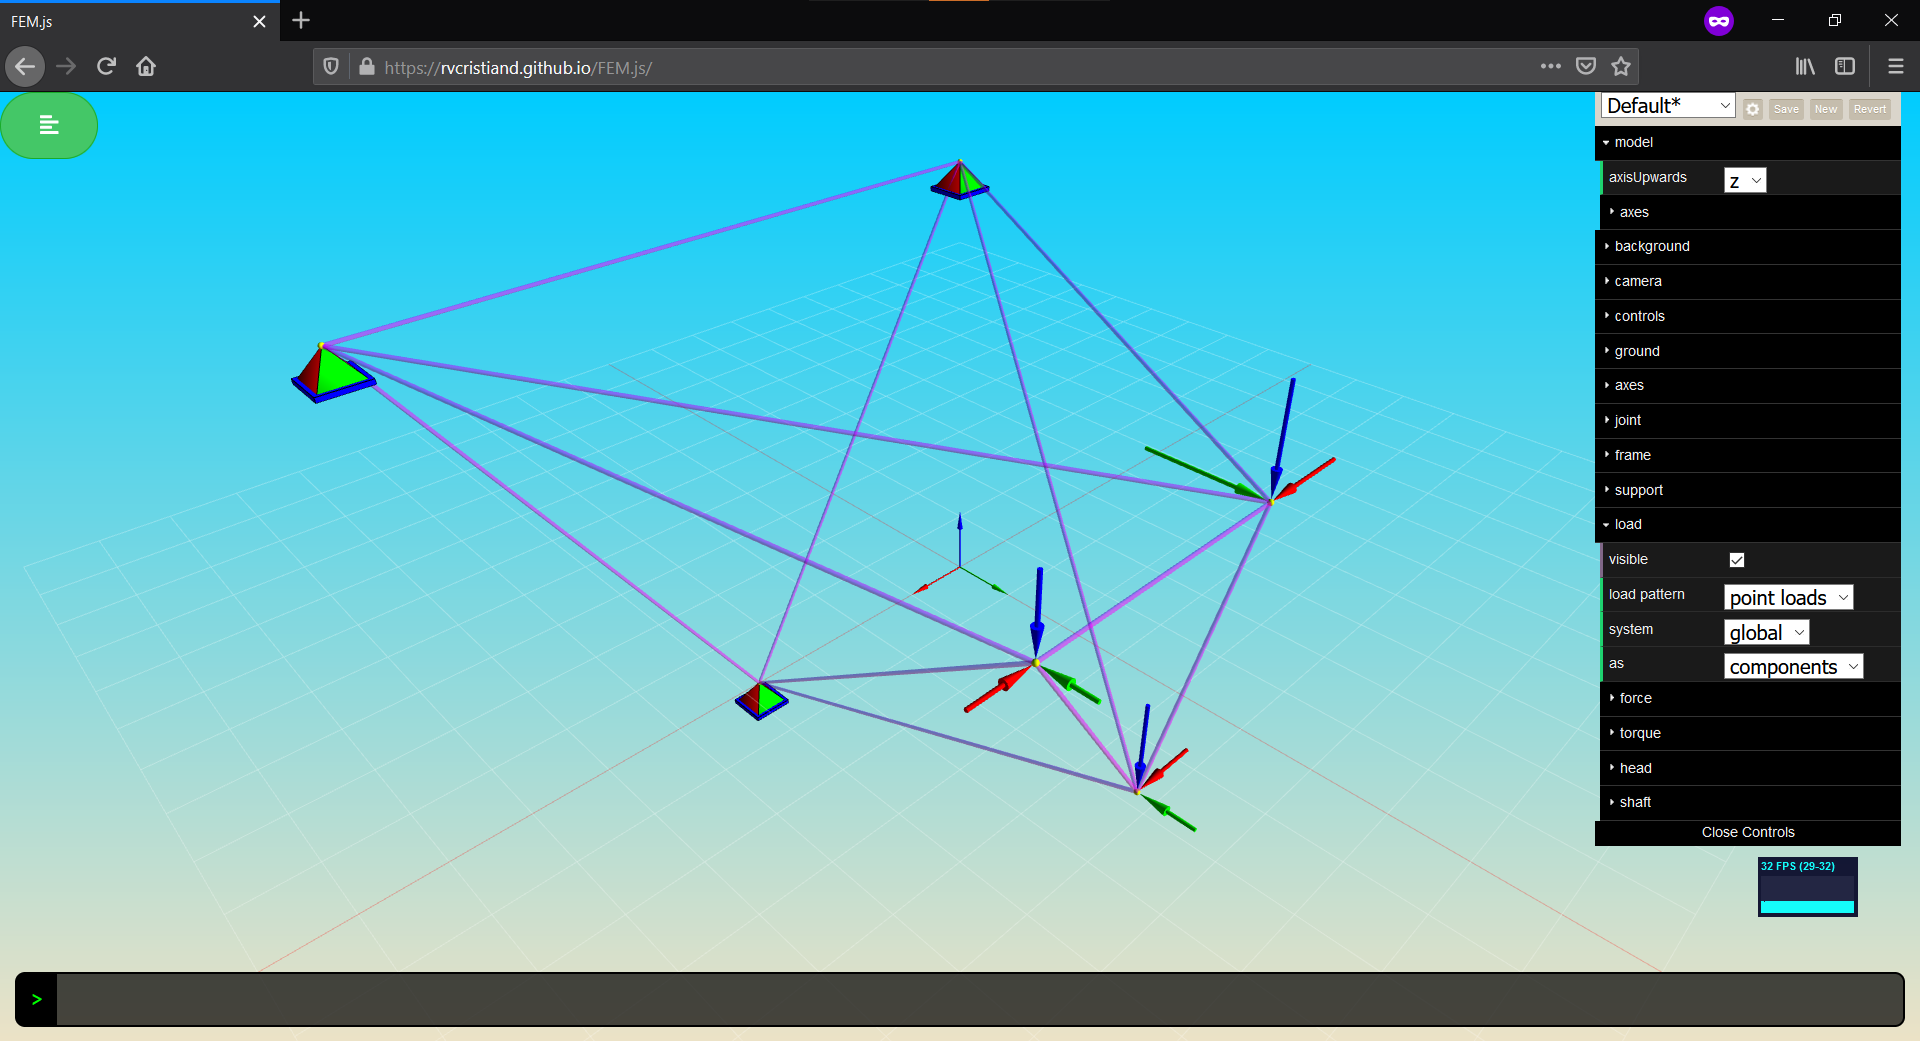
\includegraphics[width=0.8\textwidth]{FEM.js/FEM.js-setModelRotation.png}
  \caption{Eje local z de la variable \texttt{model} apuntando hacia arriba de la pantalla.}
  \label{fig:FEM.js-setModelRotation}
\end{figure}

Esto es posible mediante la función \verb|setModelRotation()|, definida en el archivo \verb|FEM.js|, que gira la variable \verb|model| cierta cantidad alrededor de un eje que pasa por su origen, de tal manera que uno de los ejes principales apunte hacia la parte de arriba de la pantalla.\\

Sin embargo, no es necesario modificar las demás variables agregadas a la variable \verb|model| para que ocupen nuevas poisciones en la escena, ya que Three.js se encarga de calcular dichas posiciones en función de su ubicación relativa en el grafo.\\

\begin{figure}[H]
  \centering
  \begin{tikzpicture}[>=stealth, every node/.style={rectangle, draw, minimum size=0.75cm}]
    \graph [tree layout, grow=right, fresh nodes, level distance=0.5in, sibling distance=0.5in]
    {
      model -- { 
        loads -- { "...", 
        "load i" -- { "frames" -- { "resultant" -- { "..." },
        "components" -- { "..." } } },
        "..." },
        frames -- { "...", 
        "frame i" -- {
          "label",
          "axes" -- { "..." },
          "extrudeFrame" -- { "edges" },
          "wireFrame" },
          "..." },
          joints -- { "...",
          "joint i" -- { "loads" -- { "...", 
          "load i" -- { "resultant" -- { "torque" -- { "..." }, 
          "force" -- { "..." } }, 
          "components" -- { "torques" -- { "..." }, 
          "forces" -- {"..."} } },
          "..." },
          "support" -- { "space" -- { "...", 
          "pin" -- { "..." },
          "pedestal" -- { "..." },
          "foundation" -- { "..." } }, 
          "analytical" -- { "rotations"-- { "x, y, z" } -- { "..." }, 
          "displacements" -- { "x, y, z" } -- { "..." } } },
          "joint" -- { "label" } },
          "..." },
          axes -- { "x, y, z" -- { "head", "straightShaft" } } } 
          };
        \end{tikzpicture}
        \caption{Grafo de la variable \texttt{model} después de agregar nodos, elementos aporticados y cargas al modelo.}
        \label{fig:FEM.js-model}
      \end{figure}
      
\pagebreak

Es evidente que la ubicación de los distintos nodos en el grafo presentado en la figura anterior obedece a la posición de estos en la escena tridimensional. Sin embargo, también han sido agrupados de manera conveniente para poder interactuar con ellos.\\

Por ejemplo, en el algoritmo \ref{alg:FEM.js-setAxesShaftLength} se presenta la implementación de la función \verb|setAxesShaft| \verb|Length()|, que modifica la longitud de las colas de las \emph{flechas} que representan un sistema coordenado. Un juego de estas flechas con el nombre \verb|axes| se agrega a la variable \verb|model| y a cada uno de los elementos aporticados (véase la figura \ref{fig:FEM.js-model}).\\

Para modificar la longitud de las colas sólo es necesario modificar su longitud a lo largo de su eje local x y actualizar la posición de la cabeza. Esto es posible gracias a que tanto la cola como la cabeza de la flecha se agregan a un objeto intermedio, \verb|x|, \verb|y| o \verb|z|, de tal manera que siempre están orientados a lo largo del eje x de dicho objeto.\\

\begin{lstlisting}[language={},caption=Implementación de la función \texttt{setAxesShaftLength()} del archivo \texttt{FEM.js}.,label=alg:FEM.js-setAxesShaftLength,frame=single]
function setAxesShaftLength( axes, length ) {
  // set axes shaft length

  axes.children.forEach( arrow => { 
    arrow.getObjectByName( 'straightShaft' ).scale.setX( length );
    arrow.getObjectByName( 'head' ).position.setX( length );
  });
}  
\end{lstlisting}
\bigskip

A través de la barra de herramientas, el usuario puede cambiar las dimensiones de las flechas de los sistemas coordenados de la variable \verb|model| y de los elementos aporticados. Varias funciones similares a esta se implementaron para interactuar con los objetos de la escena. A continuación se presentan algunas de las más relevantes.\\

\subsection{setFrameView()}

La función \verb|setFrameView()| permite ver los elementos aporticados del modelo como \emph{palillos} o extruídos, según su sección transversal.\\

En el algoritmo \ref{alg:FEM.js-setFrameView} se presenta la implementación de la función \verb|setFrameView()|. La función alterna el valor de la propiedad \verb|visible| de los objetos \verb|wireFrame| y \verb|extrudeFrame| entre falso y verdadero, para presentar los elementos aporticados en la escena en una o en otra representación.\\

\begin{lstlisting}[language={},caption=Función \texttt{setFrameView()} implementada en el archivo \texttt{FEM.js}.,label=alg:FEM.js-setFrameView, frame=single]
export function setFrameView( view ) {
  // set frame view
  
  var promise = new Promise( ( resolve, reject ) => {
    let wireframeView = view == 'wireframe', extrudeView = view == 'extrude';

    if ( wireframeView || extrudeView ) {
      model.getObjectByName( 'frames' ).children.forEach( frame => {
        frame.getObjectByName( 'wireFrame' ).visible = wireframeView;
        frame.getObjectByName( 'extrudeFrame' ).visible = extrudeView;
      });
      
      resolve( "'" + view + "' view setted" );
    } else {
      reject( new Error( "'" + view + "' does not exits" ) );
    }
  });

  return promise;
}
\end{lstlisting}
\bigskip

En la figura \ref{fig:FEM.js-setFrameView} se presenta FEM.js después de ejecutar la función \verb|open()| para abrir el archivo \verb|example_3.json|. Este archivo también ha sido generado con pyFEM para analizar el ejercicio 7.3 de \cite{escamilla1995microcomputadores}. El usuario es capaz de alternar la representación de los elementos aporticados con la barra de herramientas.\\

\begin{figure}[ht]
  \centering
  \setlength{\columnseprule}{0pt}
  
  \begin{multicols}{2}
    \begin{minipage}[b]{0.8\columnwidth}
      \centering
      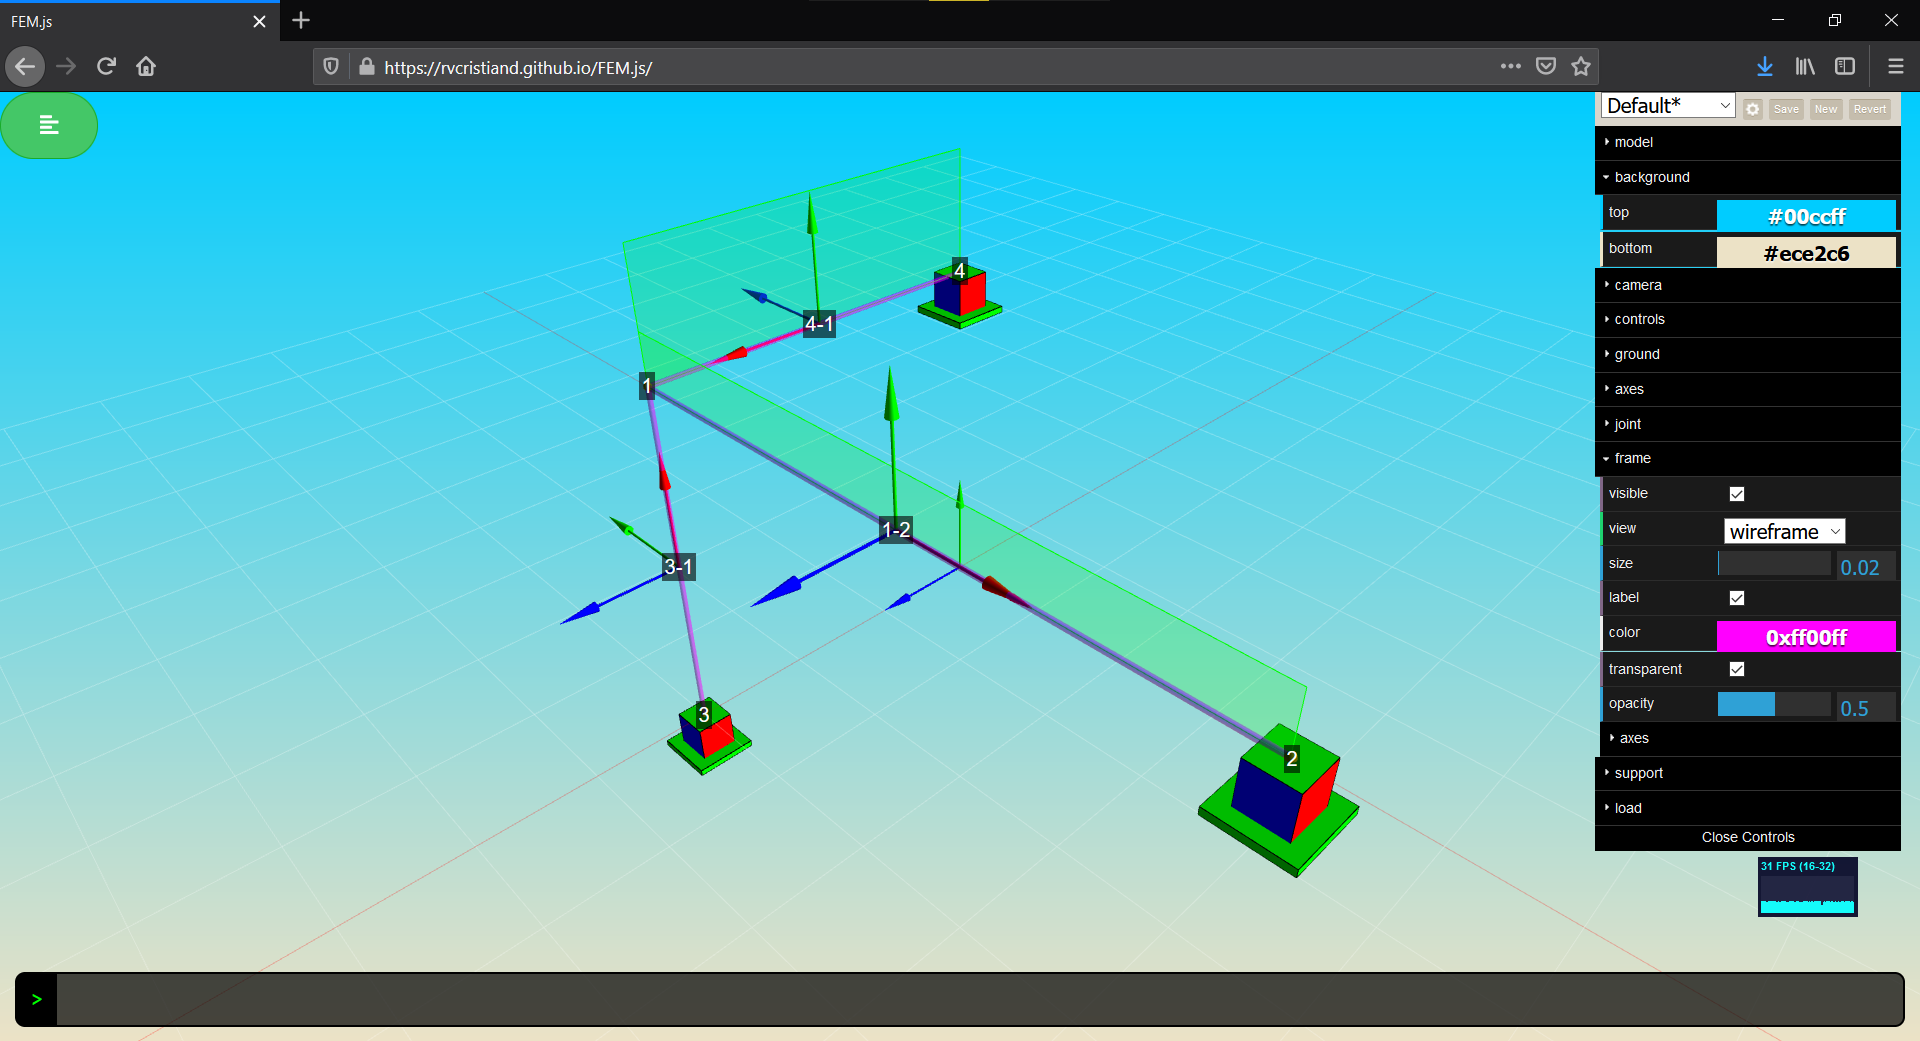
\includegraphics[width=\textwidth]{FEM.js/FEM.js-setFrameView-wireframe.png}
      Estructura de palillo.
    \end{minipage}
  
    \begin{minipage}[b]{0.8\columnwidth}
      \centering
      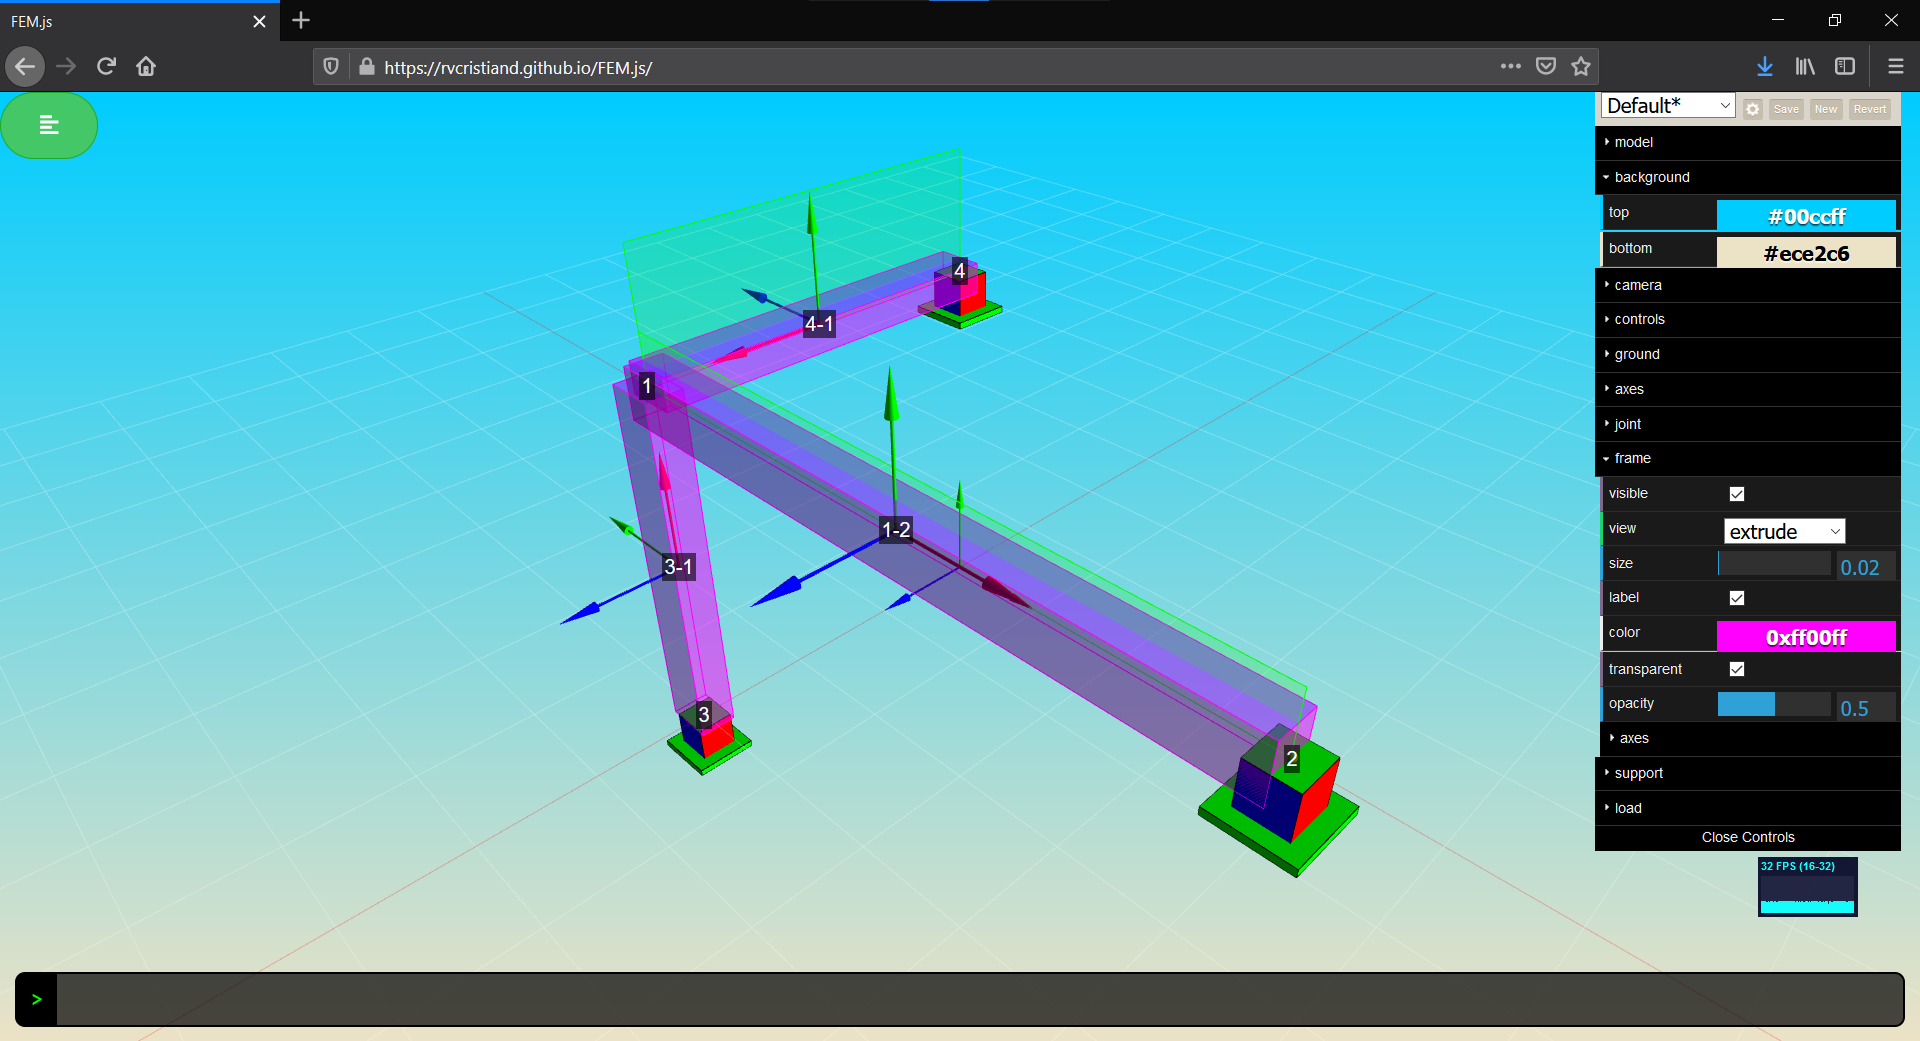
\includegraphics[width=\textwidth]{FEM.js/FEM.js-setFrameView-extrude.png}
      Estructura extruída.
    \end{minipage}
  \end{multicols}
  \caption{Representación del \texttt{example\_3.json} en \textit{estructura de palillos} o \textit{extrído}.}
  \label{fig:FEM.js-setFrameView}
\end{figure}

\subsection{setSupportMode()}

La función \verb|setSupportMode()| permite ver los apoyos del modelo como objetos tridimensionales o como flechas, según los grados de libertad restringidos.\\

En el algoritmo \ref{alg:FEM.js-setSupportMode} se presenta la implementación de la función \verb|setSupportMode()|. La función alterna el valor de la propiedad \verb|visible| de los objetos \verb|analytical| y \verb|space| entre falso y verdadero, para presentar los apoyos en la escena en una o en otra representación.\\

\begin{lstlisting}[language={},caption=Función \texttt{setSupportMode()} implementada en el archivo \texttt{FEM.js}.,label=alg:FEM.js-setSupportMode, frame=single]
function setSupportMode( mode ) {
  // set support mode

  var support;

  Object.keys( structure.supports ).forEach( name => {
    support = model.getObjectByName( 'joints' ).getObjectByName( name ).getObjectByName( 'support' );
    support.getObjectByName( 'analytical' ).visible = ( mode == 'analytical' );
    support.getObjectByName( 'space' ).visible = ( mode == 'space' );
  });
}
\end{lstlisting}
\bigskip

En la figura \ref{fig:FEM.js-setSupportMode} vuelve y se presenta el archivo \verb|example_3.json| abierto con FEM.js, donde se muestra las diferentes representaciones disponibles de los apoyos del modelo. El usuario es capaz de alternar la presentación de los apoyos con la barra de herramientas. Así mismo, es capaz de modificar las dimensiones de estos objetos.\\

\begin{figure}[ht]
  \centering
  \setlength{\columnseprule}{0pt}
  
  \begin{multicols}{2}
    \begin{minipage}[b]{0.8\columnwidth}
      \centering
      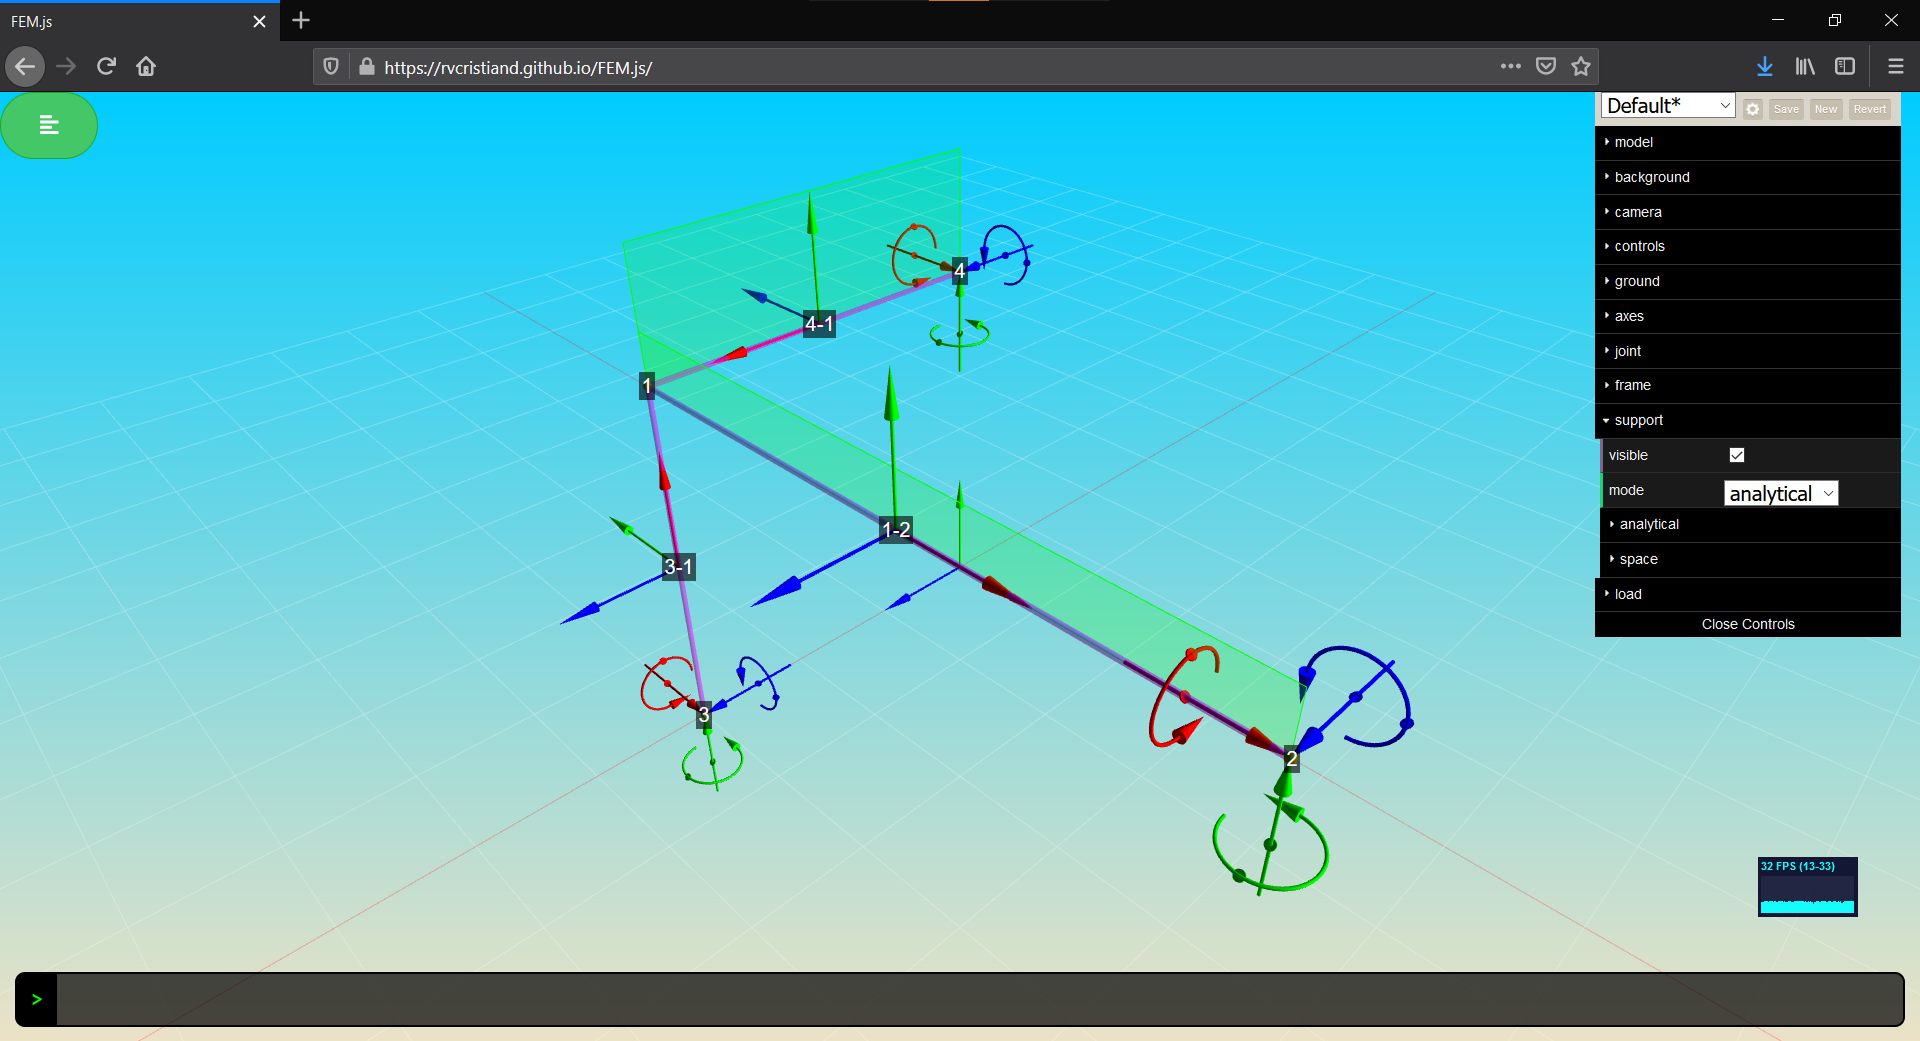
\includegraphics[width=\textwidth]{FEM.js/FEM.js-setSupportMode-analytical.png}
      Apoyos en modo \textit{analytical}.
    \end{minipage}
  
    \begin{minipage}[b]{0.8\columnwidth}
      \centering
      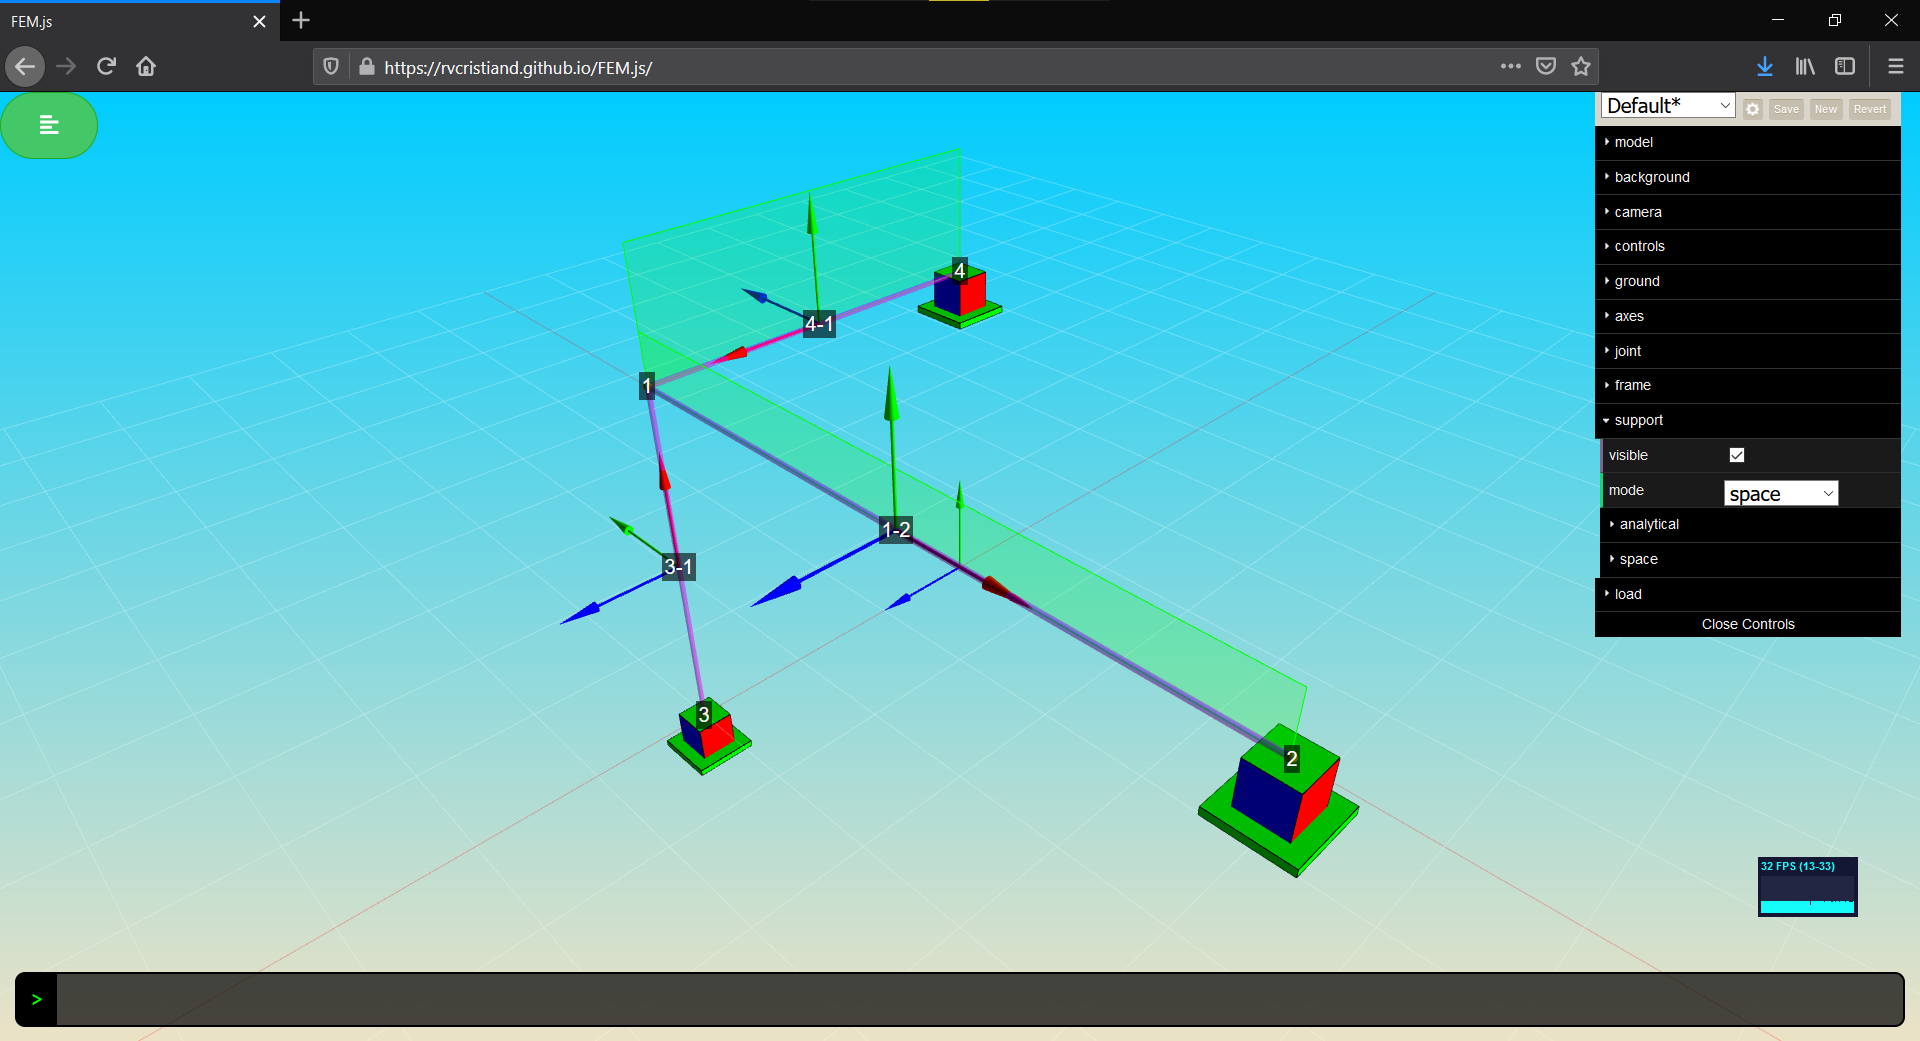
\includegraphics[width=\textwidth]{FEM.js/FEM.js-setSupportMode-space.png}
      Apoyos en modo \textit{space}.
    \end{minipage}
  \end{multicols}
  \caption{Representación de los apoyos \texttt{example\_3.json} abierto con FEM.js.}
  \label{fig:FEM.js-setSupportMode}
\end{figure}

\subsection{setLoadPatternVisible()}

La función \verb|setLoadPatternVisible()| permite alternar entre las cargas puntuales y distribuidas de los diferentes casos de carga.\\

En el algoritmo \ref{alg:FEM.js-setLoadPatternVisible} se presenta la 

